\begin{comment}
Problème NP vs #P
Théorème de Toda
Description du paper JVV
Complexité exacte vs approximative
Countage exact vs approximatif
Borne sur le comptage ("a tighter bound for counting max-weight solutions to 2SAT instances" ou l'équivalent pour 3SAT)
\end{comment}

\chapter{Complexité du comptage}
\label{cha:complexite-du-comptage}

\begin{comment}
    \subsection*{Plan}
    
    \begin{enumerate}
        \item Introduire les problèmes algorithmiques difficiles
        \item Décrire les applications de ces problèmes
        \item Expliquer les prochaines sections
        \item Expliquer pourquoi on ne parle pas des machines de Turing (thèse de Church-Turing)
    \end{enumerate}
\end{comment}

Qu'est-ce qu'un problème de comptage? Simplement, un tel problème consiste à déterminer le nombre de solutions respectant un ensemble de contraintes. Les problèmes de comptage font partie des problèmes computationnellement difficiles, ce qui signifie qu'il est peu probable que ces problèmes soient résolubles efficacement. Les problèmes de comptage surgissent dans de nombreuses disciplines, avec des applications en raisonnement probabiliste~\cite{rothHardnessApproximateReasoning1996, sangPerformingBayesianInference2005, abramsonHailfinderBayesianSystem1996}, en fiabilité des réseaux~\cite{valiantComplexityEnumerationReliability1979, duenas-osorioCountingBasedReliabilityEstimation2017}, en mécanique statistique~\cite{jerrumPolynomialtimeApproximationAlgorithms1993} et en intelligence artificielle~\cite{balutaQuantitativeVerificationNeural2019}. Contrairement à certains problèmes étudiés en algorithmie quantique, comme l'échantillonnage de bosons~\cite{aaronsonComputationalComplexityLinear2011} ou l'échantillonnage de circuits aléatoires~\cite{boulandComplexityVerificationQuantum2019}, une solution à ces problèmes peuvent avoir un impact concret, justifiant alors l'étude de tels problèmes.

Ce chapitre tente de décrire le cadre théorique entourant la classe des problèmes de comptage en détails. Pour ce faire, celle-ci est définie à l'aide du langage de la théorie de la complexité à la section~\ref{sec:classes-de-complexite}. Le problème de comptage prototypique, le problème de satisfaisabilité, sert d'exemple et est décrit à la section~\ref{sec:satisfaisabilite-booleenne}. Celui-ci est d'une grande importance pour ce projet et est ainsi référencé tout au long de ce mémoire. La section~\ref{sec:intractabilite-approximation-et-optimisation} explique l'importance des méthodes approximatives alors que la section~\ref{sec:comptage-de-modeles} décrit les solveurs modernes pour les problèmes de comptage. Finalement, le comportement des instances aléatoires pour ces problèmes est présenté à la section~\ref{sec:transitions-de-phase}, où des transitions de phase font étonnamment leurs apparitions.

Il est souvent favorable de décrire la théorie de la complexité à l'aide du concept de \textit{machine de Turing}. Cependant, ce mémoire suppose que la thèse de Church-Turing soit vraie, et donc que n'importe quel modèle de calcul puisse être utilisé de manière équivalente, pour faire abstraction de ce langage et simplifier les idées présentées.

%-----------------------------------------------------------------------------%

\section{Classes de complexité}
\label{sec:classes-de-complexite}

\begin{comment}
\subsection*{Plan}

\begin{enumerate}
    \item Définir comment quantifier la complexité d'un problème (temps contre espace)
    \item Décrire le but des classes de complexité
    \item Expliquer les propriétés des classes de complexité et leurs relations
    \item Expliquer la notation de la complexité (O notation) et les machines de Turing
    \item Décrire la tour de complexité (hiérarchie polynomiale) 
    \item Comparer les classes importantes: P et NP et \#P
    \item Établir la conjecture P != NP
    \item Mentionner le théorème de Toda
    \item Parler des classes de complexités quantique
    \item Parler de la these de church-turing pour les ordis quantiques
\end{enumerate}

\subsection*{Références}

1. Moore, Cristopher, and Stephan Mertens, The Nature of Computation (Oxford, 2011; online edn, Oxford Academic, 17 Dec. 2013), https://doi.org/10.1093/acprof:oso/9780199233212.001.0001, accessed 19 July 2024.

2. Arora, S. and Barak, B. Computational Complexity: A Modern Approach. (Cambridge University Press, Cambridge, 2009). doi:10.1017/CBO9780511804090.
\end{comment}

La théorie de la complexité s'intéresse à la classification des problèmes algorithmiques en \textit{classes de complexité}, c'est-à-dire en ensembles de problèmes de même complexité. Classifier un problème permet de caractériser les ressources nécessaires pour sa résolution par un algorithme. Les problèmes d'une même classe possèdent une difficulté inhérente similaire, ce qui permet le choix d'un algorithme et de ressources appropriées en conséquence. Savoir qu'un problème n'est pas réalistement résoluble, ou plus précisément intraitable, limite les attentes. Sachant ceci, la recherche dans cette direction peut s'avérer grandement utile. La théorie de la complexité cherche aussi à comparer les problèmes de différentes complexités. Ces comparaisons permettent de comprendre l'espace des problèmes en plus grande profondeur. Par exemple, il est évident que certains problèmes sont plus facile à résoudre que d'autres. Comparer des problèmes faciles avec des problèmes difficiles peut aider à comprendre ce qui rend un problème difficile et donc à trouver des algorithmes résolvant efficacement les problèmes plus complexes. Des liens, nommés réductions, peuvent aussi être définis au sein d'une même classe d'une complexité. Un algorithme efficace pour un problème pourrait aussi être efficace pour un problème similaire s'il existe une réduction entre ceux-ci. Les classes de complexité, de manière similaire au modèle de la machine de Turing, tentent de définir de manière abstraite la difficulté d'un problème. Peu importe le matériel informatique à notre disposition, un problème d'une classe donnée ne devrait pas changer de classe. Un problème trivial devrait rester trivial peu importe la quantité de ressources utilisée.  

Comment est-il possible de déterminer la complexité d'un problème? Pour ce faire, les classes de complexité se basent sur les ressources indispensables à la résolution du problème: le temps et la mémoire. Afin de trouver la solution à un problème, un programme doit effectuer un certain nombre d'opérations, limité dans le temps par le matériel informatique. On parle alors de \textit{complexité en temps}. Afin de produire un résultat final, le programme doit garder en mémoire les résultats intermédiaires. Ceux-ci doivent être sauvegardés dans le matériel informatique afin d'être réutilisés ultérieurement. Comme la quantité d'information conservée est aussi un facteur limitant pour le matériel informatique, on parle donc de \textit{complexité en espace}. 

La complexité en temps et en espace d'un problème est définie selon la taille de celui-ci. Afin de capturer cette dépendance, on cherche à trouver une loi d'échelle encapsulant la difficulté d'un problème en fonction de sa taille. Le temps et la mémoire quantifient bien les ressources nécessaires des algorithmes. Par contre, ceux-ci dépendent du matériel informatique utilisé. Il est attendu qu'un ordinateur moderne soit bien plus performant qu'une des premières machines analogues. Comment retirer cette dépendance de la notion de complexité? Pour ce faire, on fait appel à la notation asymptotique, communément appelé la \textit{notation $\mathcal{O}$}. La notation asymptotique caractérise la vitesse de croissance d'une fonction en ne considérant que son comportement global à l'infini. Les coefficients ainsi que les termes asymptotiquement inférieurs ne sont pas considérés. Par exemple, pour une taille de problème $n$, la résolution de celui-ci pourrait demander un temps exponentiel $\mathcal{O}(2^{n})$ et une mémoire polynomiale $\mathcal{O}(n)$. Remarquons qu'il n'y a aucune dépendance au matériel informatique: deux ordinateurs différents doivent effectuer le même nombre d'opérations et sauvegarder la même quantité d'information. Un de ces ordinateurs pourrait toutefois résoudre le problème plus rapidement si celui-ci peut effectuer un plus grand nombre d'opérations par seconde ou accéder plus rapidement à sa mémoire. L'attrait des classes de complexité vient donc en partie de cette abstraction du matériel informatique.

La quantification de ces ressources permet la séparation de plusieurs problèmes: il est en effet souhaitable d'être capable de séparer les algorithmes efficaces de ceux qui ne le sont pas. Commençons par définir deux classes de complexité particulièrement importantes: \textsf{P} et \textsf{NP}. Pour ce faire, un certain type de problème doit d'abord être défini. Un \textit{problème de décision} regroupe simplement tous les problèmes pouvant se répondre par oui ou non. Pour tout problème de décision $A$, on peut représenter celui-ci par une fonction $A(x) \in \set{ 0, 1 }$, où $x$ représente une instance du problème. Les problèmes de décision se manifestent fréquemment, tant en informatique qu'en physique. Ceux-ci se présentent sous diverses formes: Est-ce qu'un nombre $x$ est premier? La configurapportn $x$ représente-t-elle un état fondamental du système donné? Est-ce qu'il existe un chemin $x$ parcourant une seule fois toutes les villes d'une région en parcourant au maximum une distance $d$?

% \begin{maindefinition}{Problème de décision}{probleme-decision}
%     Une fonction $A(x)$ est un problème de décision si
%     \begin{align*}
%         A(x) = 
%         \begin{cases}
%            0 \text{ si } x \text{ est une réponse «non» du problème} \\
%            1 \text{ si } x \text{ est une réponse «oui» du problème}
%         \end{cases}
%     \end{align*}
% \end{maindefinition}

Quand peut-on dire qu'un problème de décision est résoluble efficacement? La classe de complexité \textsf{P}, pour « temps polynomial », tente de répondre à cette question. Informellement, un problème de la classe \textsf{P} est un problème de décision qui peut être résolu en temps polynomial. Un problème est donc considéré comme efficacement résoluble ou \textit{traitable}, s'il appartient à la classe \textsf{P}. 

\begin{maindefinition}{Classe de complexité \textsf{P}}{classe-p}
    Une fonction $A$ fait partie de la classe de complexité \textsf{P} si et seulement si elle prend la forme 
    \begin{equation*}
        A(x)=\exists y
    \end{equation*}
    et calculable en temps polynomial, c’est-à-dire en temps $O(n^{c})$ pour une taille $n = \lvert x \rvert$ et une constante $c$, où $\lvert y \rvert = \mathrm{poly}(\lvert x \rvert )$.
\end{maindefinition}

Soit, par exemple, le problème de décision du test de primalité $A$. Ce problème cherche à déterminer si un entier naturel $x$ est premier ou composé. Ce problème peut être résolu, c'est-à-dire qu'il est possible de calculer $A(x)=\exists y$, en temps polynomial $\tilde{O}(\log(n)^{12})$~\cite{PRIMESAnnalsMathematics}, où la notation $\tilde{O}$ signifie que les termes polylogarithmiques sont aussi cachés. 
% \textcolor{mydarkred}{\textit{Rajouter des exemples!}}

La relation entre un calcul en temps polynomial et un calcul efficace semble évidente de prime abord. La thèse de Cobham–Edmonds indique en effet qu'un problème algorithmique peut être résolu efficacement s'il est résoluble en temps polynomial~\cite{cobhamIntrinsicComputationalDifficulty1965, edmondsPathsTreesFlowers1965}. Cependant, certains problèmes ne possèdent pas de solutions efficaces en pratique. Par exemple, un problème peut appartenir à la classe \textsf{P}, mais être doté d'un grand coefficient limitant le calcul. Cela n'étant pas le cas pour la majorité des problèmes, cette supposition s'avère malgré tout une bonne règle empirique. 

Une deuxième classe particulièrement importante en théorie de la complexité est la classe \textsf{NP}, pour « temps polynomial non déterministe ». Celle-ci regroupe les problèmes de décision dont les solutions sont vérifiables en temps polynomial. Généralement, ces problèmes sont formulés sous la forme suivante: Existe-t-il une solution, vérifiable en temps polynomial, au problème donné? Malgré que les solutions sont vérifiables efficacement, déterminer l'existence d'une telle solution n'est pas nécessairement possible en temps polynomial. Une métaphore souvent utilisée pour la description d'un problème \textsf{NP} est celle d'une aiguille dans une botte de foin. Trouver cette aiguille parmi la quantité énorme de brins de foin est un défi de taille. Par contre, une fois l'aiguille trouvée, il n'y a aucun doute qu'il s'agit bien d'une aiguille. 

\begin{maindefinition}{Classe de complexité \textsf{NP}}{classe-np}
    Une fonction $A$ fait partie de la classe de complexité \textsf{NP} si et seulement si elle prend la forme
    \begin{equation*}
        A(x) = \exists y \mid B(x,y)
    \end{equation*}
    pour une fonction $B \in  \textsf{P}$, où $\lvert y \rvert = \mathrm{poly}(\lvert x \rvert)$.
\end{maindefinition}

On appelle $B$ le vérificateur du problème de décision $A$ et $y$ le certificat ou le témoin pour l'entrée $x$. Un exemple de problème \textsf{NP} est le problème du commis voyageur. Soit un graphe $x$ représentant les villes d'une région particulière. Est-ce que le commis voyageur peut visiter toutes les villes exactement une fois et revenir à son point de départ en parcourant une distance inférieure à $d$? Dans ce cas, la fonction $A$ détermine le chemin parcouru alors que la fonction $B$ détermine si un chemin $y$ est de taille inférieure à $d$.

La classe \textsf{NP} est aussi définie comme la classe de problèmes pouvant être résolu par une machine de Turing non déterministe en temps polynomiale, d'où son nom. Cette définition est toutefois équivalente à la définition précédente, c'est-à-dire la classe de problèmes vérifiable par une machine de Turing déterministe en temps polynomial~\cite{sipserIntroductionTheoryComputation2012}. Notons que la classe \textsf{P} est contenue dans la classe \textsf{NP}. En effet, comme un problème de \textsf{P} est résoluble en temps polynomial, alors nécessairement une solution à ce problème peut aussi être vérifiée en temps polynomial. Cependant, une question, faisant partie des problèmes du prix du millénaire~\cite{carlsonMillenniumPrizeProblems2006}, demeure ouverte: est-ce que $\textsf{P} = \textsf{NP}$? La conjecture largement répandue répond à cette question par la négative. L'hypothèse de temps exponentiel~\cite{impagliazzoComplexityKSAT2001} suggère par exemple que certains problèmes de \textsf{NP} sont résolubles en temps exponentiel, un résultat significatif sur la difficulté de ces problèmes. En conséquence, un problème est \textit{intraitable} s'il n'est pas résoluble en temps polynomial, par opposition à un problème traitable. 

% \textcolor{mydarkred}{\textit{Conséquences?}}

% \textcolor{mydarkred}{\textit{Parler de non-déterministique. Est-ce pertinent comme il faut introduire les machines de Turing non-déterministe? Autrement, un problème appartient à la classe \textsf{NP} s'il est résoluble en temps polynomial par une machine de Turing non-déterministe. }}

% \textcolor{mydarkred}{\textit{On a donc que $P \subseteq NP$.}}
% \textcolor{mydarkred}{\textit{NP pour temps non-déterministique.}}
% \textcolor{mydarkred}{\textit{La conjecture "Exponential Time Hypothesis" suggère que certains problèmes dans NP prennent un temps exponentiel.  (voir https://arxiv.org/pdf/1611.04471 pour plus d'information)}}

La classe de complexité d'intérêt dans le cadre de ce mémoire est la classe \textsf{\#P} introduit par Valiant~\cite{valiantComplexityComputingPermanent1979}. Cette classe, définie par extension à la classe \textsf{NP}, cherche non seulement à déterminer si un problème de décision possède une solution, mais aussi à spécifier le nombre de solutions à ce problème. Ainsi, un \textit{problème de comptage} consiste à trouver le nombre de solutions d'un problème de décision. Un problème de comptage est donc défini par rapport à un problème de décision. Prenons par exemple le problème du commis voyageur. Le problème de décision généralement défini cherche un trajet de taille inférieure à une certaine distance. Le problème de comptage adjoint exige alors le nombre de trajets possibles de taille inférieure à la distance donnée. 

\begin{maindefinition}{Classe de complexité \textsf{\#P}}{classe-sharp-p}
    Une fonction $A$ fait partie de la classe de complexité $\textsf{\#P}$ si et seulement si elle prend la forme
    \begin{equation*}
        A(x) = \lvert \set{ y \mid B(x, y)} \rvert
    \end{equation*}
    pour une fonction $B \in \textsf{P}$, où $\lvert y \rvert = \mathrm{poly}(\lvert x \rvert)$ pour toutes les valeurs $y$ prises par $B(x,y)$.
\end{maindefinition}

% \textcolor{mydarkred}{\textit{Changer!}}

Par définition, un problème de la classe \textsf{\#P} est au moins aussi difficile qu'un problème de la classe \textsf{NP}. Connaître le nombre de solutions à un problème de décision indique effectivement s'il existe au moins une solution à un problème de décision. Cependant, les problèmes de comptage intéressants possèdent fréquemment un nombre exponentiel de solutions, impliquant une plus grande complexité inhérente.

% \textcolor{mydarkred}{\textit{Donc exponentiellement plus difficile que NP?}}

Comme que les problèmes de la classe \textsf{P} font aussi partie de la classe \textsf{NP}, et que les problèmes de cette dernière appartiennent aussi à la classe \textsf{\#P}, il est nécessaire de définir un concept supplémentaire spécifiant la difficulté d'un problème au sein d'une classe. Intuitivement, un problème est \textit{difficile} pour une classe de complexité s'il est au moins aussi difficile que tous les problèmes de la classe. Plus formellement, un problème difficile pour une classe donnée signifie qu'il existe une \textit{réduction}, c'est-à-dire une transformation en temps polynomial d'un problème à un autre, entre ce problème et tous les autres problèmes de la classe. De plus, un problème est \textit{complet} s'il est difficile et aussi membre de la classe. La figure~\ref{fig:complexity-classes} éclaircit ces concepts. Les problèmes complets d'une classe représentent alors les problèmes les plus difficiles de celle-ci. Par exemple, le problème du commis voyage est dit \textsf{NP}-complet, car il fait partie des problèmes considérés comme difficile de la classe \textsf{NP}. Il est toutefois crû que celui-ci ne fasse pas partie de la classe \textsf{P} selon la conjecture $\textsf{P} \neq \textsf{NP}$.

\begin{figure}[h!]
    \centering
    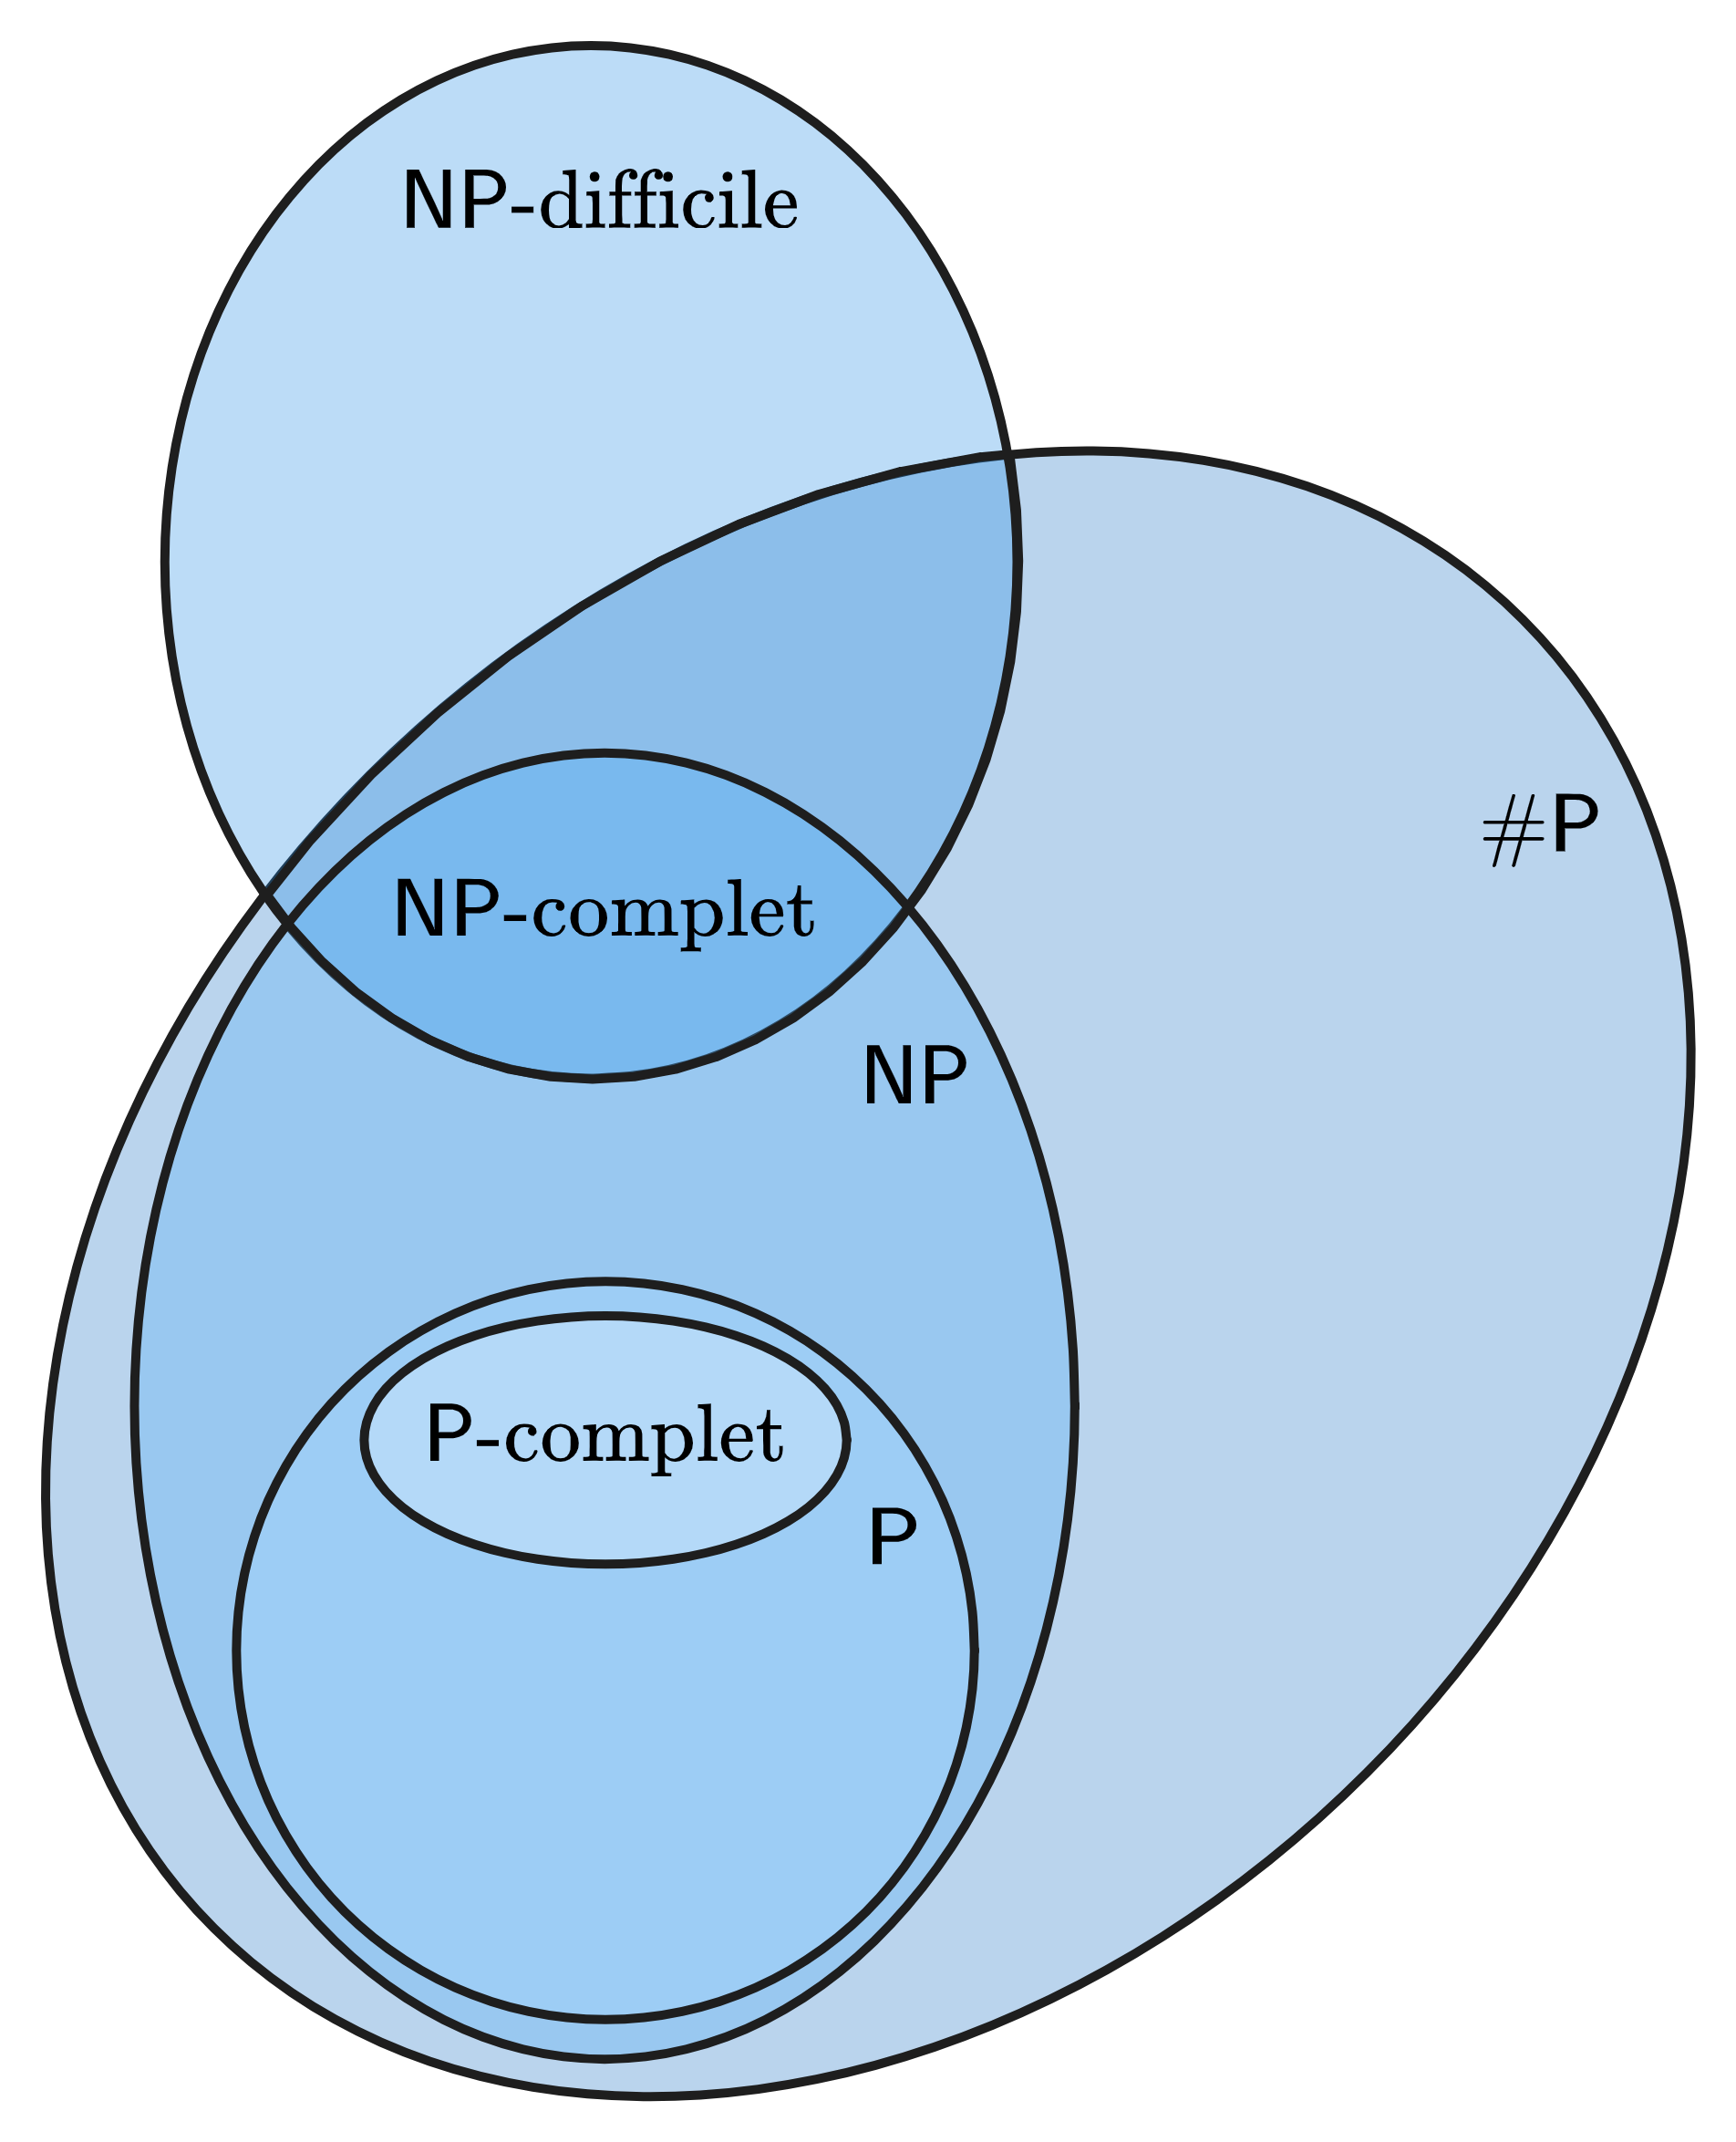
\includegraphics[width=0.4\textwidth]{figures/complexity-classes.png}
    \caption[Classes de complexité]{Classes de complexité.}
    \label{fig:complexity-classes}
\end{figure}

L'importance des problèmes \textsf{\#P} au sein de la théorie de la complexité s'observe entre autres par le théorème de Toda~\cite{todaPPHardPolynomialTime1991}. Ce résultat marquant montre que tous les problèmes de la hiérarchie polynomiale \textsf{PH} peuvent être résolus en temps polynomial avec un oracle résolvant instantanément les problèmes \textsf{\#P}. La hiérarchie polynomiale généralise les classes de complexité \textsf{P}, \textsf{NP} et \textsf{co-NP} en capturant les classes de problèmes exprimés par une alternance de quantificateurs d'existence ($\exists$) ou d'universalité ($\forall$) (voir la définition~\ref{def:classe-np} pour un exemple contenant un seul quantificateur d'existence). Ainsi, cette hiérarchie \textsf{PH} est comprise dans la classe de complexité $\textsf{P}^{\textsf{\#P}}$, c'est-à-dire les problèmes résolubles avec un oracle \textsf{\#P}. Comme la hiérarchie polynomiale contient de nombreux problèmes importants, ce théorème suggère l'incroyable puissance des problèmes de comptage.

\begin{subtheorem}{Théorème de Toda}{toda}
    La hiérarchie polynomiale \textsf{PH} est contenue dans $\textsf{P}^{\textsf{\#P}}$.
\end{subtheorem}

% \textcolor{mydarkred}{\textit{https://www.cs.cornell.edu/~sabhar/chapters/ModelCounting-SAT-Handbook-prelim.pdf}}

% L'ordinateur quantique boulverse le domaine de la complexité classique. En effet, la thèse de Church-Turing, stipulant qu'un algorithme est calculable si et seulement s'il est calculable par une machine de Turing, ne prend pas en compte les processus physiques. Le principe de Church-Turing-Deustch généralise la thèse de Church-Turing en énoncçant qu'un dispositif de calcul universel peut simuler n'importe quel processus physique. \textcolor{mydarkred}{\textit{Enlever?}}

L'ordinateur quantique bouleverse le domaine de la complexité classique. Les problèmes autrefois intraitables deviennent potentiellement résolubles efficacement à l'aide d'algorithmes quantiques. Deux nouvelles classes de complexité font alors leurs apparitions pour décrire les problèmes résolubles à l'aide de matériel informatique quantique. La classe \textsf{BQP} généralise la classe \textsf{BPP}, pour « temps polynomial probabiliste à erreur bornée », c'est-à-dire la classe de problèmes résoluble avec une probabilité d'erreur inférieure à $1/3$, pour les ordinateurs quantiques. De plus, la classe de complexité \textsf{QMA}, pour « Merlin Arthur Quantique » se définit par rapport à la classe \textsf{BQP} de manière analogue à la classe \textsf{NP} pour la classe \textsf{P}. La théorie de la complexité quantique étudie les classes de complexité quantiques dans l'objectif de déterminer les problèmes où les algorithmes quantiques comportent un avantage par rapport aux algorithmes classiques. Ce mémoire avance la recherche dans cette direction en étudiant la performance des algorithmes quantiques en comparaison avec les algorithmes classiques.

% Entre, le principe de Church-Turing-Deutsch fût proposée comme une version plus forte de la thèse de Church-Turing en utilisant les lois de la physique. 

% \textcolor{mydarkred}{\textit{Définir les problèmes de décision et de comptage ainsi que les classes de complexité de manière plus formelle (alphabet, )? Changer $B(x,y)$ par $xBy$?}}

% \textcolor{mydarkred}{\textit{Expliquer plus le théorème de Cook-Levin.}}

% \textcolor{mydarkred}{\textit{Discuter des relations entre les classes de complexité définies.}}

% \textcolor{mydarkred}{\textit{Church-Turing-Deutch}}
% \textcolor{mydarkred}{\textit{Parler des problèmes d'optimisation combinatoire.}}

% \textcolor{mydarkred}{\textit{Ajouter une figure sur les classes de complexité.}}
% \textcolor{mydarkred}{\textit{Classe PP}}
% \textcolor{mydarkred}{\textit{Classes de complexité quantique}}

%-----------------------------------------------------------------------------%

\section{Satisfaisabilité booléenne}
\label{sec:satisfaisabilite-booleenne}

\begin{comment}
\subsection*{Plan}

\begin{enumerate}
    \item Introduire SAT
    \item Énumérer certaines applications de ce problème
    \item Faire le lien entre le problème de décision SAT et le problème de comptage SAT
    \item Introduire NAE3SAT et 1in3SAT
    \item Énoncer la réduction entre NAE3SAT/1in3SAT et 3SAT
    \item Introduire la transition de phase critique de ces problèmes
    \item Expliquer pourquoi prendre la version positive de ces problèmes n'est pas un problème
    \item Parler du comptage des problèmes SAT
    \item Introduire la transition de phase critique de ces problèmes
\end{enumerate}

\subsection*{Références}

1. Moore, Cristopher, and Stephan Mertens, The Nature of Computation (Oxford, 2011; online edn, Oxford Academic, 17 Dec. 2013), https://doi.org/10.1093/acprof:oso/9780199233212.001.0001, accessed 19 July 2024.

2. Arora, S. and Barak, B. Computational Complexity: A Modern Approach. (Cambridge University Press, Cambridge, 2009). doi:10.1017/CBO9780511804090.

3. Achlioptas, D., Chtcherba, A., Istrate, G. and Moore, C. The phase transition in 1-in-k SAT and NAE 3-SAT. Proceedings of the Annual ACM-SIAM Symposium on Discrete Algorithms (2001) doi:10.1145/365411.365760.
\end{comment}

Le problème de \textit{satisfaisabilité booléenne} ou problème SAT est particulièrement important dans la théorie de la complexité. Montré comme \textsf{NP}-complet par le théorème de Cook-Levin~\cite{cookComplexityTheoremprovingProcedures1971,levinUniversalSequentialSearch}, il fut à la base de la définition de \textsf{NP}-complétude et du problème $\textsf{P} \stackrel{?}{=} \textsf{NP}$. Celui-ci est aussi couramment utilisé dans la preuve de réductions de problèmes au sein de la classe de complexité \textsf
{NP}. Le problème SAT a une multitude d'applications, comme le diagnostic des fautes d'un circuit logique ou la planification en intelligence artificielle~\cite{marques-silvaPracticalApplicationsBoolean2008}, en partie grâce à la facilité de formuler ces applications à l'aide de formules propositionnelles.

Une \textit{formule propositionnelle}, ou une expression booléenne, est un ensemble de variables booléennes, $x_{i} \in \set{\textsc{\texttt{FAUX}}, \textsc{\texttt{VRAI}}}$, reliées par des opérateurs booléens de conjonctions (\textsc{\texttt{OU}}, $\lor$), de disjonctions (\textsc{\texttt{ET}}, $\land$) ainsi que de négation (\textsc{\texttt{NON}}, $\neg$).  Un \textit{littéral} désigne dans ce contexte une variable booléenne ou sa négation. Par exemple, l'expression $(x_{1} \land x_{2}) \lor \neg x_{3}$ est une formule booléenne composée des variables $x_{1}$, $x_{2}$ et $x_{3}$, ainsi que des littéraux $x_{1}$, $x_{2}$ et $\neg x_{3}$. Notons que l'équivalence $\textsc{\texttt{FAUX}} \leftrightarrow 0$ et $\textsc{\texttt{VRAI}} \leftrightarrow 1$ est utilisée dans ce mémoire par commodité.

Un problème SAT se décrit par une formule propositionnelle. Résoudre le problème consiste à déterminer s'il existe une combinaison de variables qui rend la formule logiquement vraie, c'est-à-dire tel que l'évaluation de celle-ci donne 1. Une telle formule est alors dite satisfaisable.

\begin{maindefinition}{Problème SAT}{probleme-sat}
    Soit une constante $n \geq 1$ et une formule propositionnelle $\varphi(x_{1}, x_{2}, \dots, x_{n})$ où $x_{i} \in \set{ 0, 1 }$.  Existe-t-il une assignation des variables $x_{1}, x_{2}, \dots, x_{n}$ telle que $\varphi$ soit satisfaisable, c'est-à-dire que $\varphi(x_{1}, x_{2}, \dots, x_{n})=1$?
\end{maindefinition}

Dans l'étude du problème SAT, les formules propositionnelles sont souvent exprimées en \textit{forme normale conjonctive} (« Conjunctive Normal Form ») (CNF). On parle alors de formules CNF. Celles-ci consistent en une conjonction d'une ou de plusieurs \textit{clauses}, où une clause est une disjonction d'un ou plusieurs littéraux. Cela implique que toute clause doit contenir au moins un littéral évaluant à 1 pour que la formule soit satisfaisable. Toute formule propositionnelle peut être réécrite en forme normale conjonctive en utilisant les lois de l'algèbre booléenne.

\begin{example}{Problème SAT}{probleme-sat}
    La formule CNF
    \begin{equation*}
        \varphi(x_{1}, x_{2}, x_{3}) = (x_{1} \lor x_{3}) \land (\neg x_{1} \lor x_{2} \lor \neg x_{3}) 
    \end{equation*}
    est satisfaisable car $\varphi(1,0,0) = (1 \lor 0) \land (\neg 1 \lor 0 \lor \neg 0) = 1$. Au contraire, la formule CNF
    \begin{equation*}
        \varphi(x_{1})= (x_{1}) \land (\neg x_{1})
    \end{equation*}
    n'est pas satisfaisable car $\varphi (x_{1}) = 0$ peu importe le choix de $x_{1}$.
\end{example}

% \textcolor{mydarkred}{\textit{Tables de vérité?}}

Le problème kSAT constitue un cas spécial du problème SAT, où le nombre de littéraux appartenant à chaque clause d'une formule CNF est restreint à $k$ littéraux au maximum. Notons que le problème kSAT est trivial pour $k=1$, résoluble en temps linéaire pour $k=2$~\cite{kromDecisionProblemClass1967}, et \textsf{NP}-complet pour $k \geq 3$~\cite{karpReducibilityCombinatorialProblems1972}. Surprenamment, les problèmes de comptage correspondant, \#2SAT et \#3SAT, appartiennent tous les deux à la classe \textsf{\#P}-complet~\cite{valiantComplexityEnumerationReliability1979}. Ainsi, compter le nombre de solutions à un problème \textsf{NP}-complet peut être difficile même s'il est possible de trouver une solution efficacement.

Dans ce mémoire, deux variantes de 3SAT seront portées à l'étude: le problème Pas-Tous-Égaux 3SAT (« Not-All-Equal 3-Satisfiability ») (NAE3SAT) et le problème 1-dans-3 3SAT (« One-in-Three 3-Sastisfiability ») (1-in-3SAT). 
Comme le problème SAT, ces problèmes appartiennent aussi à la classe de complexité \textsf{NP}-complet. Les versions monotones de ces problèmes, où la négation de variables n'est pas permise, sont étonnamment aussi \textsf{NP}-complet par le théorème de dichotomie de Schaefer~\cite{schaeferComplexitySatisfiabilityProblems1978}. Ces problèmes de décision peuvent être associés aux problèmes de comptage \#NAE3SAT et \#1-in-3SAT de la classe de complexité \textsf{\#P}.

\begin{maindefinition}{Problème NAE3SAT}{probleme-nae3sat}
    Soit une formule CNF $\varphi(x_{1}, x_{2}, \dots, x_{n})$ pour laquelle chaque clause $C$ contient au maximum 3 littéraux. Existe-t-il une assignation des variables $x_{1}, x_{2}, \dots, x_{n}$ telle que $\varphi$ soit satisfaisable tout en s'assurant que tous les littéraux de chaque clause $C$ ne soient pas égaux?
\end{maindefinition}

Notons qu'un problème NAE3SAT peut être décrit par un problème 3SAT. Soit une formule CNF $f$ exprimant un problème 3SAT. Une formule CNF $g$, représentant le problème NAE3SAT associé à $f$, est construite en transformant chaque clause $(x \lor y \lor z)$ de $f$ en $(x \lor y \lor z) \land (\neg x \lor \neg y \lor \neg z)$. Cette nouvelle contrainte renforce alors la condition supplémentaire, c'est-à-dire que les littéraux de chaque clause ne peuvent être tous égaux. Cette relation illustre bien une symétrie cachée derrière le problème NAE3SAT; chacune des variables possèdent en moyenne la même probabilité d'être vraie ou fausse.

\begin{maindefinition}{Problème 1-in-3SAT}{probleme-1in3sat}
    Soit une formule CNF $\varphi(x_{1}, x_{2}, \dots, x_{n})$ pour laquelle chaque clause $C$ contient au maximum 3 littéraux. Existe-t-il une assignation des variables $x_{1}, x_{2}, \dots, x_{n}$ telle que $\varphi$ soit satisfaisable tout en s'assurant qu'exactement un littéral de chaque clause $C$ soit logiquement vrai?
\end{maindefinition}

De la même façon que pour le problème NAE3SAT, le problème 1-in-3SAT se transforme en un problème 3SAT en transformant chaque clause $(x \lor y \lor z)$ en $(x \lor y \lor z) \land (x \lor \neg y \lor \neg z) \land (\neg x \lor y \lor \neg z) \land (\neg x \lor \neg y \lor z) \land (\neg x \lor \neg y \lor \neg z)$, de manière à encoder la contrainte additionnelle du problème 1-in-3SAT.

% \textcolor{mydarkred}{\textit{Parler du nombre de solutions.}}

%-----------------------------------------------------------------------------%

\section{Intraitabilité, approximation et optimisation}
\label{sec:intractabilite-approximation-et-optimisation}

\begin{comment}
\subsection*{Plan}

\begin{enumerate}
    \item Expliquer le concept d'intractabilité
    \item Montrer la difficulté de résoudre des problèmes computationnels de manière exacte
    \item Expliquer les advantages des méthodes approximatives (temps polynomial, applications réelles)
    \item Introduire rigoureusement le concept d'approximation
\end{enumerate}

\subsection*{Références}

Subhash Khot. Inapproximability of NP-complete Problems, Discrete Fourier Analysis, and Geometry. In Proceedings of the International Congress of Mathematicians 2010 (ICM 2010)
\end{comment}

Les problèmes algorithmiques des classes de complexité \textsf{NP}-difficile et \textsf{\#P}-difficile sont considérés comme intraitables en raison de leur complexité intrinsèque. En effet, il est improbable qu'un algorithme puisse résoudre exactement ces problèmes en temps polynomial. Par exemple, bien que certaines instances du problème SAT contenant plus d'un million de variables sont résolubles efficacement, d'autres instances de moins d'un millier de variables ne peuvent être résolus par les solveurs de pointe~\cite{froleyksSATCompetition20202021}. Cette difficulté s'accentue pour le problème \#SAT, où même une centaine de variables peut s'avérer trop complexe. 

L'intraitabilité de tels problèmes mène alors à un paradigme différent; Sachant qu'il est irréaliste de résoudre certains problèmes exactement, est-ce qu'il est possible de trouver une solution approximative de manière efficace? L'exactitude des solutions est alors sacrifié pour une performance accrue.

Les problèmes de décision ne possédant que deux solutions, oui ou non, il n'est pas possible de fournir une solution approximative. Un \textit{problème d'optimisation}, défini en conjonction à un problème de décision, est alors une notion plus adéquate pour incorporer la notion d'approximation. Ces problèmes ne cherchent plus à trouver la solution optimale, mais plutôt à obtenir une réponse suffisamment près de la valeur optimale. Un exemple de problème d'optimisation, particulièrement étudié dans le domaine de l'optimisation quantique en raison de sa simplicité d'implémentation sur du matériel informatique quantique, est le problème de coupe maximum (­« Maximum Cut ») (Max-Cut). Ce problème cherche une coupe séparant les sommets d'un graphe en deux ensembles complémentaires tel que le nombre d'arêtes séparant les deux ensemble soit maximal. Le problème Max-Cut étant \textsf{NP}-complet, il est difficile d'obtenir une coupe optimale, mais une coupe sous-optimale peut possiblement être trouvée efficacement.

Un problème d'optimisation $\Pi$ est constitué d'un ensemble d'instances valides $I_{\Pi}$, où chaque instance $x \in I_{\Pi}$ possède un ensemble de solutions faisables $S_{\Pi}(x)$. Une fonction objectif $\text{obj}_{\Pi}$, aussi nommée fonction de coût ou de perte, quantifie la qualité d'une solution approximative $y$ de $x$ en lui assignant un nombre réel. En conséquence, résoudre approximativement un problème d'optimisation correspond à minimiser ou maximiser la fonction de coût. Une mesure de succès fréquemment utilisée, autant classiquement que quantiquement, est le \textit{rapport d'approximation},
\begin{equation}
    \alpha(x, y) = \frac{\text{obj}_{\Pi}(x, y)}{\text{OBJ}_{\Pi}(x)} \,,
\end{equation}
où $\text{OBJ}_{\Pi}(x) = \min_{y} \text{obj}_{\Pi} (x, y)$. Ce type de problème est formalisé sous le nom de problème d'optimisation \textsf{NP}, mais une définition détaillée est évitée ici par simplicité. Bien que les algorithmes d'approximation heuristiques offrent fréquemment de bons résultats, ceux-ci ne possèdent aucune garantie quant à la qualité de ces solutions.

Pour pallier ce problème, des algorithmes approximatifs avec garantis sont définis en fonction de deux paramètres: la tolérance $\varepsilon$ et la confiance $\delta$. La tolérance indique l'erreur multiplicative maximale de l'approximation et la confiance indique la probabilité de succès de l'algorithme. Ce couple de paramètres est souvent utilisés pour décrire les algorithmes approximatifs.

Un \textit{algorithme d'approximation de tolérance $\varepsilon$} pallie ce problème en garantissant une solution optimale à une erreur multiplicative près~\cite{vaziraniApproximationAlgorithms2003}. Pour un problème de minimisation $\Pi$, cet algorithme $f$ produit une solution $s$ pour toutes instances $x \in I_{\Pi}$ tel que $f_{\Pi}(x, y) \leq \varepsilon(\lvert x \rvert ) \cdot \text{OBJ}(x)$ où $\lvert  x \rvert $ est la taille de l'instance et $\varepsilon \geq 1   $. Cette définition peut être détendue en permettant à l'algorithme de produire une telle solution avec une certaine probabilité. Cette variante, l'\textit{algorithme d'approximation randomisé de tolérance $\varepsilon$}, introduit des concepts pertinents pour le chapitre~\ref{cha:echantillonnage-quasi-uniforme-comptage-approximatif-randomise}.

% \textcolor{mydarkred}{\textit{What is $f$?}}

\begin{subtheorem}{Algorithme d'approximation randomisé}{algorithme-approximation-randomise}
    Un algorithme d'approximation randomisé de tolérance $\varepsilon$ pour un problème de minimisation $\Pi$ est un algorithme aléatoire prenant en entrée une instance $x \in D_{\Pi}$ et une tolérance $\varepsilon$ et qui produit une solution $y \in S_{\Pi}(x)$ tel que
    \begin{equation*}
        \mathrm{ Pr } [f_{\Pi}(x, y) \leq \varepsilon(\lvert x \rvert ) \cdot \text{OBJ}(x)] \geq \frac{1}{2}
    \end{equation*}
    en temps polynomial.
\end{subtheorem}

Ces algorithmes se généralisent facilement pour un problème de maximisation.
En relaxant la condition d'exactitude, il est attendu qu'un gain en possible en terme d'efficacité. Cependant, cela n'est pas toujours aussi clair. Il existe en effet certains problèmes où trouver une solution approximative en haut d'un certain rapport d'approximation demeure intraitable tel le problème de couverture par ensembles~\cite{lundHardnessApproximatingMinimization1994}. Les algorithmes d'approximation s'appliquent aussi aux problèmes de comptage, tel que présenté à la section~\ref{sec:comptage-approximatif-randomise}.

%-----------------------------------------------------------------------------%

\section{Comptage de modèles}
\label{sec:comptage-de-modeles}

\begin{comment}
\subsection*{Plan}

\begin{enumerate}
    \item Décrire les résultats actuels en terme de comptage exact et approximatif
    \item Énumérer les algorithmes et les solveurs modernes (DPLL, \textit{survey propagation}, \textit{belief propagation})
    \item Mentionner les meilleures bornes sur les problèmes de comptage
    \item https://arxiv.org/pdf/2002.06879
    \item Lien avec la fonction de partition
\end{enumerate}

\subsection*{Références}

1. Wahlström, M. A Tighter Bound for Counting Max-Weight Solutions to 2SAT Instances. in Parameterized and Exact Computation (eds. Grohe, M. and Niedermeier, R.) 202–213 (Springer, Berlin, Heidelberg, 2008). doi:10.1007/978-3-540-79723-419.

2. Sinclair, A. and Jerrum, M. Approximate counting, uniform generapportn and rapidly mixing Markov chains. Information and Computation 82, 93–133 (1989).
\end{comment}

% est-il possible de préciser sa complexité dans le pire des cas? Une quantité signifiante de travaux s'intéresse à cette question.

Sachant désormais que le comptage est un problème difficile, comment résoudre celui-ci? Le comptage des solutions d'une formule propositionnelle est spécifiquement connu dans la littérature sous le nom de \textit{comptage de modèles}. De nombreuses méthodes, autant exactes qu'approximatives, ont été développées pour sa résolution~\cite{biereHandbookSatisfiabilityVolume2009}. 

Les méthodes exactes attaquent généralement le problème en explorant exhaustivement l'espace des solutions possibles, de manière similaire à l'algorithme de Davis-Putnam-Logemann-Loveland (DPLL) pour les problèmes SAT~\cite{davisMachineProgramTheoremproving1962}. Les algorithmes de recherche locale pour SAT, tel l'algorithme WalkSAT, peuvent aussi être étendus pour résoudre \#SAT. Toutefois, les solveurs les plus performants actuellement sont basés sur les réseaux de tenseurs, un object mathématique provenant du domaine de la matière condensée~\cite{kourtisFastCountingTensor2019, dudekEfficientContractionLarge2020, dudekParallelWeightedModel2021}. Ces réseaux sont utiles dans de nombreux autres domaines et sont d'ailleurs utilisés dans ce travail pour la simulation de circuit quantique et font donc l'objet de l'annexe~\ref{ann:simulation-circuits-quantiques-avec-reseaux-de-tenseurs}. Bien que différents développements accentuent la taille des systèmes résolubles exactement, les solveurs ont de la difficulté à trouver l'ensemble de solutions de l'espace de recherche. 

Les méthodes approximatives allègent ce problème à l'aide d'heuristiques fournissant des estimations avec ou sans garanties. Plusieurs applications du comptage ne nécessitent pas un résultat exact; distinguer la différence entre $10^{30}$ et $10^{30}+1$ solutions n'est pas toujours pertinent. L'algorithme de Stockmeyer, qui approxime le nombre de solutions à un facteur deux avec un nombre polynomial d'appels à un oracle \textsf{NP} en s'appuyant sur les fonctions de hachage, fut un pas majeur pour le comptage approximatif~\cite{stockmeyerComplexityApproximateCounting1983}. Plusieurs modifications ont propulsé le domaine vers des performances accrues de sorte que la majorité des méthodes modernes se basent effectivement sur les fonctions de hachage. Cependant, une méthode alternative due à Jerrum, Valiant et Vazirani utilise plutôt la relation entre l'échantillonnage aléatoire de solutions et le comptage approximatif pour résoudre le problème. Malgré l'originalité de cette idée, la recherche dans cette direction s'est estompée en raison de la difficulté de l'échantillonnage de solutions avec les conditions nécessaires. Ce travail relance cette possibilité en pourvoyant une nouvelle façon d'échantillonner avec les algorithmes variationnels quantiques. Une discussion approfondie est présentée au chapitre~\ref{cha:echantillonnage-quasi-uniforme-comptage-approximatif-randomise}.

Les avancées en physique, tel les réseaux de tenseurs, présentent des avantages pour le comptage de modèle, mais l'inverse est aussi vrai. Le problème du comptage est intimement reliée au domaine de la mécanique statistique. En effet, déterminer la fonction de partition d'un système à température nulle est en réalité équivalent à un problème de comptage~\cite{timmeCountingComplexDisordered2009}. Considérons la fonction de partition $Z$ pour un Hamiltonien $H$ où l'énergie fondamentale est fixée à $E_{0} = 0$,
\begin{equation}
    Z = \sum_{i} e^{-\beta E_{i}} \,,
\end{equation}
où $\beta = \frac{1}{k_{b} T}$, $k_{B}$ est la constante de Boltzmann et $T$ est la température. Dans la limite $T \to 0$, les seuls termes non-nuls de la somme sont $e^{-\beta E_{0}}$, c'est-à-dire les termes associés aux états fondamentaux du système. Ainsi, pour un système dégénéré de $N_{0}$ états fondamentaux, la fonction de partition devient $Z = N_{0}$. Calculer la fonction de partition correspond ainsi à déterminer le nombre d'états fondamentaux.

Le développement du calcul quantique a aussi mené à de fructueux aboutissements. L'algorithme de comptage quantique prend avantage de l'algorithme de Grover et de l'algorithme d'estimation de phase quantique pour approximer le nombre de solutions à l'aide de $(\sqrt{\frac{N}{M}})$ itérations, où $M$ est le nombre de solutions, de taille exponentielle pour les problèmes SAT et $N$ est le nombre d'états possibles~\cite{brassardQuantumCounting1998}. Le nombre d'itérations nécessaires profite ainsi d'un gain quadratique par rapport à la complexité optimale classique de $O(\frac{N}{M})$.

Notons que dans tous les cas, le comptage de solutions aux formules CNF, l'objet de ce travail, ne s'effectue jamais en temps polynomial. Même les approches approximatives nécessitent un nombre exponentiel d'opérations, indiquant davantage la difficulté de ce problème.


% \textcolor{mydarkred}{\textit{Model counting!}}
% \textcolor{mydarkred}{\textit{Hashing based}}
% \textcolor{mydarkred}{\textit{JVV}}
% \textit{}
% \textcolor{mydarkred}{\textit{Permanent}}

% \textcolor{mydarkred}{\textit{Quantum counting?}}

% \textcolor{mydarkred}{\textit{https://www.scottaaronson.com/papers/apxcount.pdf}}

% \textcolor{mydarkred}{\textit{https://www.cs.cornell.edu/~sabhar/chapters/ModelCounting-SAT-Handbook-prelim.pdf}}

% \textcolor{mydarkred}{\textit{https://www.cs.toronto.edu/~meel/Papers/handbook-chapter.pdf}}

% \textcolor{mydarkred}{\textit{Partition function}}

%-----------------------------------------------------------------------------%

\section{Transitions de phase}
\label{sec:transitions-de-phase}

\begin{comment}
\subsection*{Plan}

\begin{enumerate}
    \item Expliquer les différentes transitions de phase et leurs intuitions
    \item Décrire l'objectif des algorithmes classiques locaux et globaux, comme le "belief propagation" ou le "survey propagation"
    \item Expliquer brièvement où se situe VQCount par rapport à ça
\end{enumerate}

\subsection*{Références}

1. Watrous, J. Quantum Computational Complexity. Preprint at https://doi.org/10.48550/arXiv.0804.3401 (2008).

2. Mézard, M. and Montanari, A. Information, Physics, and Computation. (Oxford University Press, Oxford, New York, 2009).

2. https://www.sciencedirect.com/science/article/pii/S0378437109010656

3. Survey propagation: An algorithm for satisfiability - Braunstein - 2005 - Random Structures amp; Algorithms - Wiley Online Library. https://onlinelibrary.wiley.com/doi/abs/10.1002/rsa.20057.
\end{comment}

La complexité d'une instance aléatoire d'un problème \textsf{NP} n'est pas toujours équivalente. En réalité, certaines instances sont résolubles en temps polynomial, alors que d'autres sont intraitables. Les discussions autour des classes de complexité s'intéressent principalement à la complexité dans le pire des cas pour décrire la difficulté inhérente d'un problème. Cependant, certaines instances peuvent posséder une complexité inférieure, pouvant alors être pris en avantage par certains algorithmes. 

Pour les problèmes SAT, la difficulté d'une instance aléatoire est grandement dépendante sur le rapport $\alpha = \frac{m}{n}$, où $m$ est le nombre de clauses et $n$ est le nombre de variables. Intuitivement, cette difficulté provient de l'ajout de contraintes au problème sous la forme de clauses. Plus surprenamment, la complexité d'une telle instance suit une transition de phase nommée \textit{transition de phase critique}. En effet, il existe une valeur critique $\alpha_{c}$ où les instances du problème SAT passe de satisfaisable à insatisfaisable dans la limite asymptotique de $n$. La difficulté du problème SAT est maximale juste avant cette transition. Pourquoi est-ce le cas?

Plusieurs autres transitions de phase existent avant la transition critique telle qu'illustré à la figure~\ref{fig:transitions-de-phase}. Ces transitions, similairement aux transitions de phase du modèle d'Ising, correspondent à des changements dans l'organisation de l'ensemble des solutions. Pour décrire cette réorganisation, une mesure de similarité est nécessaire pour comparer les différentes entrées au problème SAT. La \textit{distance de Hamming} entre deux chaînes de bits de même taille correspond au nombre de positions dans les chaînes où les bits correspondants diffèrent. 


Avant la première transition de phase, la \textit{transition de phase de regroupement}, toutes les solutions d'une instance du problème SAT sont situées au sein du même amas, chacune à une distance d'Hamming polynomiale selon la taille de l'instance. \textcolor{mydarkred}{\textit{Compléter.}}

% \textit{transition de phase de congélation}

\begin{figure}[h]
    \centering
    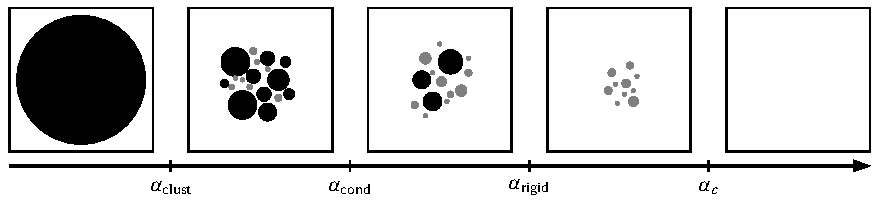
\includegraphics[width=1\textwidth]{figures/phase-transitions.pdf}
    \caption[Transitions de phase du problème SAT]{Schéma des transitions de phase du problème SAT selon le rapport du nombre de clauses au nombre de variables $\alpha$. Les transitions de phases illustrées sont la transition de regroupement $\alpha_{\text{clust}}$, la transition de condensation $\alpha_{\text{cond}}$, la transition de congélation $\alpha_{\text{rigid}}$ et la transition de satisfaisabilité $\alpha_{c}$.}
    \label{fig:transitions-de-phase}
\end{figure}

Les approches locales semblent échouer à la transition de condensation, alors que la difficulté du problème SAT semble provenir de la transition de congélation. La transition de phase critique pour NAE3SAT est situé à $\alpha_{c} \approx 2.1$~\cite{achlioptasPhaseTransition1ink2001} et à $\alpha_{c} \approx 2/3$~\cite{raymondPhaseDiagram1in32007} pour 1-in-3SAT. Les instances du problème \#1-in-3SAT près du seuil critique appartiennent à la catégorie des problèmes bloqués. Les problèmes \#P dans ce régime sont parmi les plus difficiles~\cite{zdeborovaStatisticalPhysicsHard2008}.

% \textcolor{mydarkred}{\textit{Pourquoi transition dynamique?}}

% \textcolor{mydarkred}{\textit{Parler du nombre de solutions.}}

% \textcolor{mydarkred}{\textit{Locked problems.}}


% \textcolor{mydarkred}{\textit{Voir papier de stefanos fast counting, plus d'informations et de références.}}

% \textcolor{mydarkred}{\textit{Algorithme local vs global}}